% ============================================================
% 4.5 ADJUSTED MARKS -- Writer: Ignacio Gimeno -- about 320 words
% THIS ANSWERS IDRIS'S QUESTION: "Have you tried the suggestion in the previous
% feedback? and see if it makes GPA more equal?"  Answer it explicitly, with a
% real-life example (his Progress Report feedback asked for one).
% Numbers: results/adjusted_mark_stats.json, results/adjusted_mark_field_distribution.csv,
% results/final_figures_stats.json (fig7), figures/final/CAPTIONS.md (entry fig7).
% ============================================================

\subsection{Adjusted Marks Halve the Inequality}
\label{sec:res-adjusted}

\guide{Ignacio -- Paragraph: a worked example a reader can picture}{%
\textbf{Give one concrete case (Idris asked for a real-life result):} take a Nursing graduate and a Business administration graduate in the same university. Explain with the numbers of Figure~\ref{fig:field-effects} what their adjusted marks would be: on average Nursing grades sit $0.53$ points above the university-year average and Business administration $0.32$ below it (\texttt{results/final\_fig1\_field\_effects.csv}), so two students with the same raw mark, say 7.5, end up about $7.0$ and $7.8$ after adjustment -- 0.85 points apart, in favour of the Business student. In the method the deviation is the university's own past one, so the exact numbers vary by university; say that. Keep it simple and use the university's past deviation, as the method does.}
\budget{90}{Ignacio}

\guide{Ignacio -- Paragraph: the answer to Idris (Table~\ref{tab:adjusted}, Figure~\ref{fig:adjusted})}{%
\textbf{Claim:} yes -- the adjusted mark makes access much more equal, provided the deviation is estimated for each university.\\
\textbf{Numbers:} distance from equal access $G$: 11.8 pp with raw marks; 7.4 with the shared field deviation ($-37\%$); 5.1 with the university's average past deviation ($-57\%$), 95\% intervals 11.0--12.6 vs 4.8--5.3; upper bound with the same year's deviation 3.6 ($-69\%$). Nursing median 40.6\% $\to$ 13.0\%; Business administration 5.4\% $\to$ 19.5\%.\\
\textbf{Interpretation:} the ranking of the variants follows the prediction results in \S\ref{sec:res-prediction}: the better a correction predicts the deviation, the more equal the selection.}
\budget{120}{Ignacio}

% Table 3 -- adjusted marks. Numbers from results/adjusted_mark_stats.json
% (checked 20 Nov 2026). Evaluation 2016-2023, 595 university-years, 79 universities.
\begin{table}[t]
\centering
\caption{\capguide{Ignacio -- say: distance $G$ from equal access (equation~\eqref{eq:gap}), graduate-weighted, percentage points, 95\% interval from 1,000 bootstrap resamples of universities; medians across university-years for two fields; deviations estimated from earlier years except the last row (upper bound, not usable in practice); 2016--2023, 595 university-years.}}
\label{tab:adjusted}
\small
\setlength{\tabcolsep}{3.5pt}
\begin{tabularx}{\linewidth}{@{}>{\raggedright\arraybackslash}X c c c c@{}}
\toprule
Mark used for ranking & $G$ (pp) & 95\% CI & Nursing & Business \\
 & & & (\%) & adm.\ (\%) \\
\midrule
Raw mark & 11.8 & 11.0--12.6 & 40.6 & 5.4 \\
Minus shared field deviation & 7.4 & 7.1--7.7 & 14.4 & 17.7 \\
Minus university's deviation last year & 5.0 & 4.7--5.3 & 12.7 & 20.0 \\
Minus university's average past deviation & 5.1 & 4.8--5.3 & 13.0 & 19.5 \\
Minus same-year deviation (bound) & 3.6 & 3.4--3.8 & 12.8 & 20.5 \\
\bottomrule
\end{tabularx}
\end{table}


\begin{figure}[t]
  \centering
  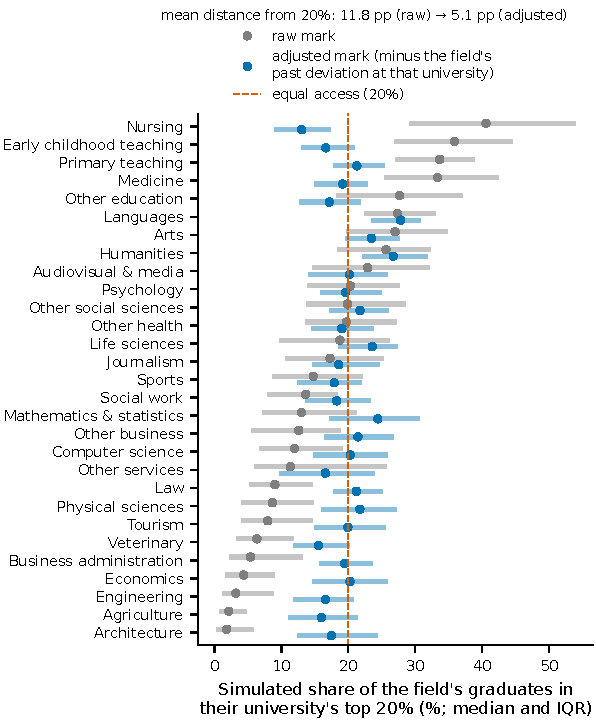
\includegraphics[width=\linewidth]{fig7_adjusted_marks}
  \caption{\capguide{Ignacio -- see CAPTIONS.md, entry "Figure 7" (file fig7): Figure~\ref{fig:selection} repeated with adjusted marks (minus the field's average past deviation at that university); median and interquartile range; 2016--2023, 595 university-years, so raw values differ slightly from Figure~\ref{fig:selection}; dashed line = equal access.}}
  \label{fig:adjusted}
\end{figure}

\guide{Ignacio -- Paragraph: why the adjusted mark is not enough on its own}{%
\textbf{Observation:} even with the same-year deviation (field means made equal), the median Nursing share is 12.8\% while Languages (27.8\%), Humanities (26.8\%) and Mathematics \& statistics (25.0\%) stay above 20\% (\texttt{adjusted\_mark\_field\_distribution.csv}, method \texttt{oracle\_current}). Equal means do not give equal access because fields differ in the \emph{spread} of their grades: a field with a narrow spread has few graduates in the upper tail. Evidence: median within-field standard deviation 0.44 points for Nursing (the narrowest) against 0.84 for Humanities and 0.87 for Languages (the widest) (\texttt{adjusted\_mark\_by\_field.csv}, column \texttt{median\_within\_field\_sd}).\\
\textbf{Consequence:} a correction must remove differences in spread as well as in level -- which is what ranking within the degree does (\S\ref{sec:res-rules}).\\
\textbf{Also say:} the 2016--2023 sample differs from Figure~\ref{fig:selection}, so the raw medians differ slightly (Nursing 40.6\% here, 41.1\% there).}
\budget{110}{Ignacio}
